\documentclass[11pt]{article}
\usepackage[margin=0.78in]{geometry}
\usepackage{amsmath,amssymb}
\usepackage{booktabs}
\usepackage{graphicx}
\usepackage{xcolor}
\usepackage{hyperref}
\usepackage{tikz}
\usetikzlibrary{arrows.meta,positioning,shapes.geometric,fit,calc,matrix}
\hypersetup{colorlinks=true,linkcolor=blue!45!black,urlcolor=blue!55!black}
\setlength{\parindent}{0pt}
\setlength{\parskip}{0.55em}
\newcommand{\status}[1]{\textbf{Status: #1}}
\newcommand{\artifact}[1]{\texttt{\detokenize{#1}}}
\newcommand{\schematicnote}{\textit{This is a schematic, not evidence.}}
\newcommand{\lookat}{\textbf{What to look at.} }
\newcommand{\caveat}{\textbf{Caveat.} }
\newcommand{\bottomline}{\textbf{Bottom line.} }
\newcommand{\codeword}[1]{\texttt{#1}}
\definecolor{trusted}{HTML}{1B9E77}
\definecolor{broken}{HTML}{D73027}
\definecolor{caution}{HTML}{E6AB02}
\definecolor{muted}{HTML}{777777}
\definecolor{gpu}{HTML}{7570B3}

\title{Why Frontier Production Starts with One Golden Snapshot\\\large Prove the assembled pipeline before multiplying it 161 times}
\author{GOTHAM PDF reconstruction notes}
\date{June 2026}

\begin{document}
\maketitle
\status{The argument for one golden run is strong. The run itself is still pending.}

\section{What we are trying to explain}

The reducer has passed synthetic tests, GPU tests, real-shard tests, and a
four-GPU/eight-shard comparison. Why not launch all 161 snapshots immediately?

Because the remaining failures would hit every snapshot the same way. If the
HIP build, complete-snapshot checks, 1024-rank reduction, output identity, or
MI250X performance is wrong, a production array does not give 161 independent
experiments. It repeats the same mistake 161 times.

\section{The simple picture}

The parts have passed tests. The assembled production machine has not.

Run one exact, complete snapshot with archived controls. Make it exercise the
whole assembled path and expose performance. Then start production at concurrency one,
using the first larger 256-node snapshot as a second scale canary.

\section{The cartoon version}

\begin{figure}[ht]
\centering
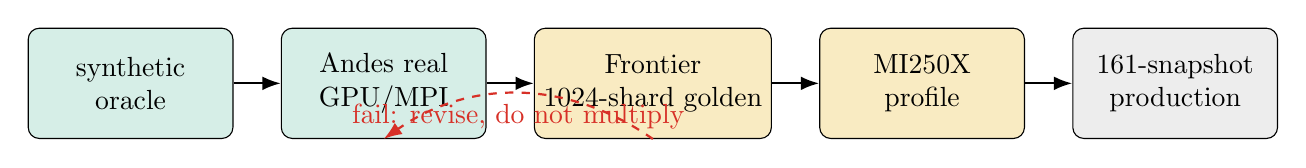
\begin{tikzpicture}[>=Latex,node distance=5mm and 6mm,
gate/.style={draw,rounded corners,align=center,minimum width=26mm,minimum height=14mm},
pass/.style={gate,fill=trusted!18}, wait/.style={gate,fill=caution!24},
future/.style={gate,fill=black!7}]
\node[pass] (synthetic) {synthetic\\oracle};
\node[pass,right=of synthetic] (andes) {Andes real\\GPU/MPI};
\node[wait,right=of andes] (golden) {Frontier\\1024-shard golden};
\node[wait,right=of golden] (profile) {MI250X\\profile};
\node[future,right=of profile] (prod) {161-snapshot\\production};
\foreach \a/\b in {synthetic/andes,andes/golden,golden/profile,profile/prod}
  \draw[->,thick] (\a)--(\b);
\draw[->,thick,broken,dashed] (golden.south) to[bend right=35]
 node[below]{fail: revise, do not multiply} (andes.south);
\end{tikzpicture}
\caption{Each gate removes a failure mode that the previous gate cannot test.
\schematicnote}
\end{figure}

The important arrow is the one pointing backward. A failed golden run sends us
back to the tested Andes path; it does not fan out into production.

\section{The more precise version}

The golden case is not an arbitrary sample. It is the exact 8 pc snapshot with
archived controls and a manageable 128-node footprint:
\begin{center}
\begin{tabular}{ll}
\toprule
Simulation / phase & \codeword{res\_8pc / phase2} \\
Source cube & \codeword{00028} \\
Archived PDF identity & \codeword{00062} at \(10.520002963096713\) \\
Expected source cycle & \(202829\) \\
Source shards / Frontier ranks & \(1024\) \\
Frontier nodes & \(128\) \\
Expected domain volume & \(400^3\) code-volume units \\
\bottomrule
\end{tabular}
\end{center}

For archived control histogram \(A\) and rebuilt histogram \(R\),
\[
E_{\rm L1}=\frac{\sum_b|R_b-A_b|}{\sum_b|A_b|},\qquad
E_{\rm total}=\frac{|\sum_bR_b-\sum_bA_b|}{\sum_b|A_b|}.
\]
The absolute-weight denominator is necessary because flux histograms are
signed.

The implemented global AMR checks require contiguous shards, unique logical
leaf keys, no ancestor/descendant pair, and the expected total volume. That is
substantially stronger than a partial run. It is not yet a mathematical proof
that every physical region is covered exactly once; geometry-to-key checks are
still needed to exclude a compensating hole and overlap.

A job exit code is not enough. The golden run passes only if all of the
following are true:
\begin{enumerate}
  \item a frozen executable checksum, source revision, and product catalog;
  \item exact contiguous shard manifest and matching complete header digests;
  \item valid records, hydro state, unique AMR leaves, no ancestor overlap;
  \item leaf-volume closure to \(400^3\) within relative tolerance \(2\times10^{-9}\);
  \item exact output number and exact float64 archived PDF time;
  \item publication accepted only when the final manifest and validator report
        both exist;
  \item passing archived \codeword{output29} radial and \codeword{output31}
        controls, including \(E_{\rm L1}<2\times10^{-5}\) for the
        \codeword{output29} radial marginal and \(E_{\rm L1}<2\times10^{-3}\)
        for full \codeword{output31};
  \item repaired \codeword{output29} angle populated rather than copied from the
        corrupted archive;
  \item predeclared acceptable \codeword{original}, \codeword{science}, and
        \codeword{all} throughput, memory, and walltime on MI250X.
\end{enumerate}

That is the gate. Anything less is a partial success.

\section{What this idea predicts}

\begin{itemize}
  \item The complete golden run should pass the declared archived-control
        limits. Similarity to the partial real-data errors is a useful
        diagnostic, not the release definition.
  \item It should disagree with the broken full \codeword{output29} while
        matching its radial marginal.
  \item It should activate and pass global checks deliberately skipped by
        partial runs.
  \item If the all-product path is atomic-bound, the original repair set may
        pass while science/all throughput requires optimization.
  \item A failed golden run should block every production array, even if the
        failure occurs after hours of otherwise plausible output. This is a
        proposed property; the current submitter does not enforce it.
\end{itemize}

\section{What the evidence actually shows}

\begin{figure}[ht]
\centering
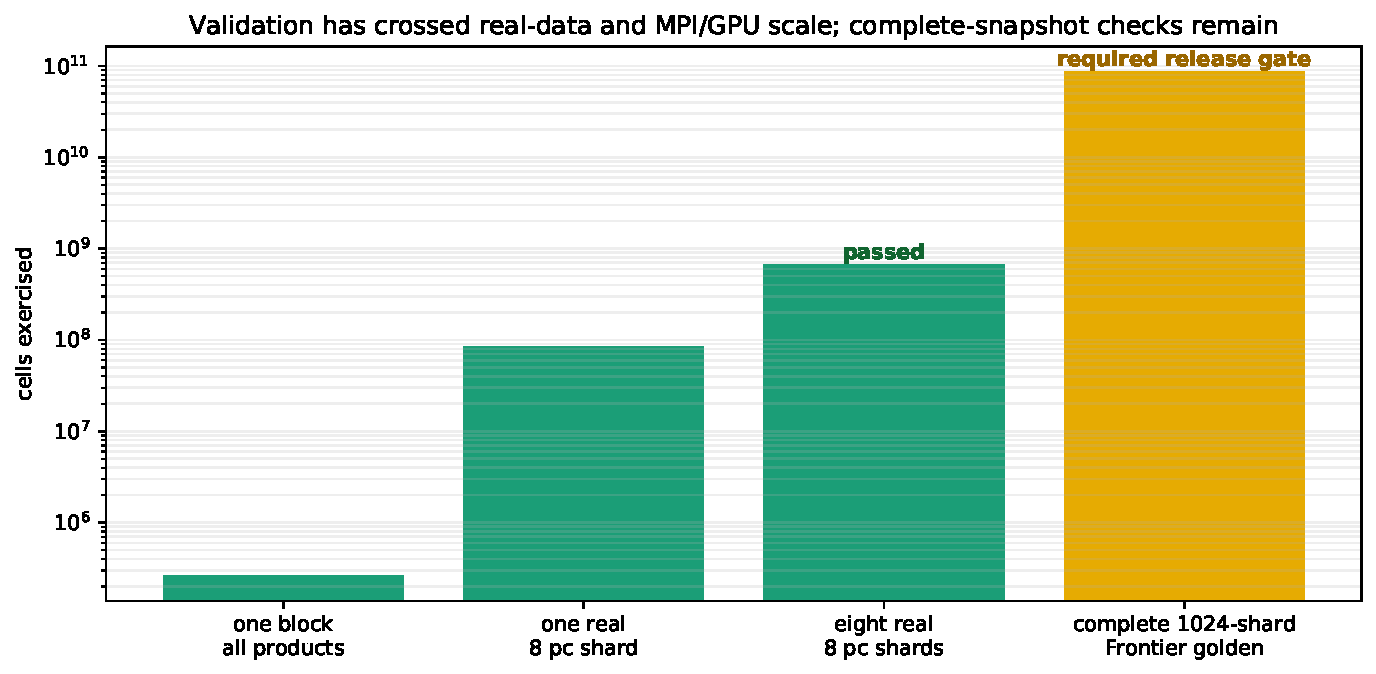
\includegraphics[width=0.94\linewidth]{figures/validation_ladder.pdf}
\caption{The validation ladder built from completed artifacts and the pending
golden requirement. The final cell count is an exact fixed-record inventory
from live source-file sizes, not a measured completed run.}
\end{figure}

\lookat The green steps are finished. The first amber step crosses a new line:
for the first time, the code can check the whole AMR volume against its
implemented logical-key and volume invariants. The earlier steps test
equations, format parsing, GPU execution, and a partial MPI reduction. They do
not see the whole domain. The pending step contains exactly 86,467,149,824
cells by live fixed-record inventory; that is scale, not a completed result.

\caveat The green steps tell us the equations and partial pipeline are
behaving. They do not certify a complete production snapshot. The partial-run
log explicitly says that global AMR closure is skipped for intentionally
limited input.

\begin{figure}[ht]
\centering
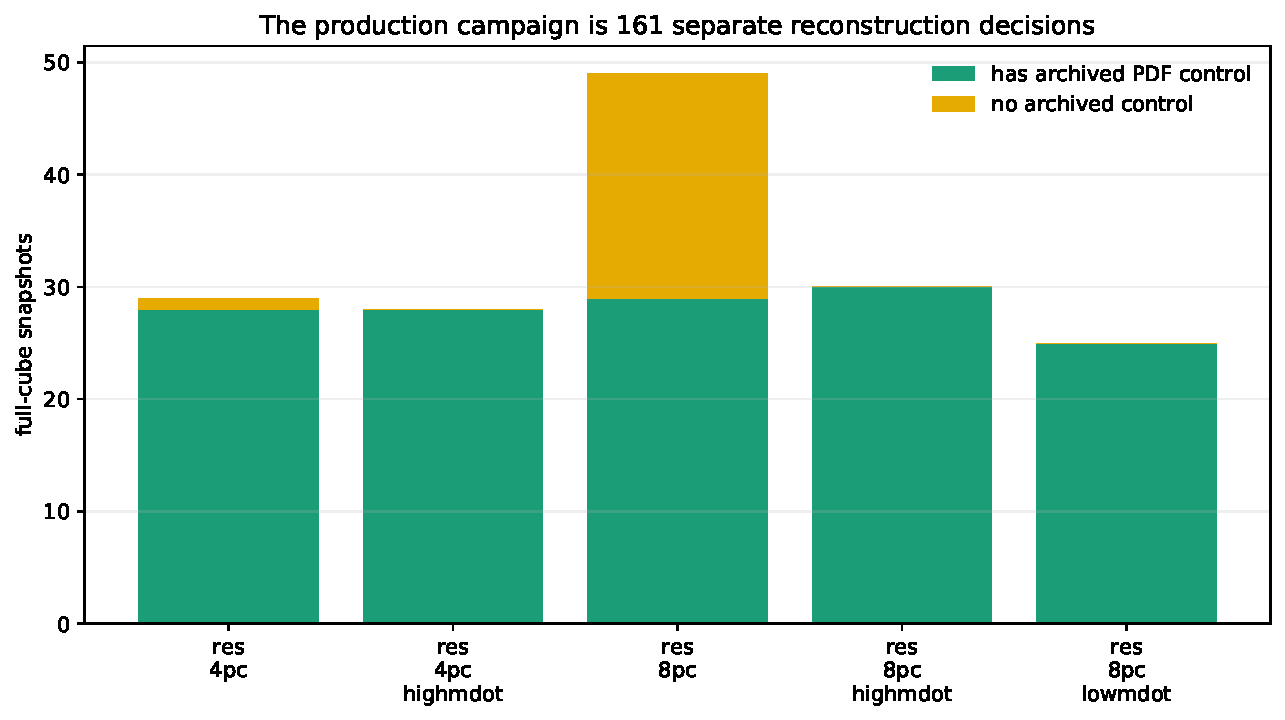
\includegraphics[width=0.94\linewidth]{figures/production_inventory.pdf}
\caption{Static Frontier inventory. There are 161 full cubes. 140 have matching
archived PDF identities and exact times; 21 uniform-phase snapshots do not.}
\end{figure}

\lookat Look at the yellow part of the \codeword{res\_8pc} bar. Those 21
snapshots lack archived PDF controls, so they depend more heavily on the
internal invariants and on confidence earned from the controlled golden run.
For those snapshots, there is no archived answer to rescue us after the fact.
The pipeline has to earn trust before they run.

\section{The key figures}

The ladder shows the missing test plainly: none of the completed steps sees the
whole domain. The inventory shows the exposure being protected. The corruption
document's control-error figure gives us reason to expect the golden controls
to pass, but not permission to skip them.

\section{What works}

\begin{itemize}
  \item The synthetic/reference and release-gate suite records six passing tests.
  \item One-block CPU/GPU agreement is near roundoff.
  \item One complete real shard and eight complete real shards have run.
  \item The four-GPU/eight-shard job completed with exit code \codeword{0:0}.
  \item The matched real-data controls pass by orders of magnitude.
  \item Static manifests map 140 source cubes to exact archived PDF identities.
  \item Jobs default to plan mode, refuse existing output, and require explicit
        confirmation tokens.
\end{itemize}

\section{What does not work}

Frontier HIP has not been built and run. No 1024-rank reduction has completed.
No complete-snapshot AMR report exists. The all-product path has not
been profiled on MI250X. Frontier filesystem behavior is unknown. Some 4 pc
snapshots require 256 nodes, twice the golden node count.
No numerical performance budget currently defines ``acceptable,'' and the
validator does not yet enforce every exact output-identity field described by
the proposed gate.

More importantly, the current gate is advisory. The golden job runs only the
lightweight manifest check and tells the operator to run
\codeword{validate\_real\_8pc.py}; the production submitter does not require a
passing golden JSON report or tie it to an executable checksum. Routine
production jobs also do not execute the 140 mapped archived controls.

So the golden snapshot is necessary, but it is not permission for high
concurrency. The first 256-node snapshot and at least one no-control uniform
snapshot remain explicit canaries.

\section{How this could be wrong}

Maybe this is overkill. If the complete run taught us nothing that the
eight-shard test had not already shown, then spending 128 nodes on a gate would
be ceremony. But the complete run is the first test that can catch missing
shards, duplicate logical leaves, ancestor/descendant pairs, a wrong total
domain volume, failures in the 1024-rank reduction, and actual Frontier
throughput. It cannot yet exclude every arbitrary physical hole or overlap.

The opposite risk is treating one golden success as universal proof. It is not.
The five simulations share schema and code, but differ in size and phase
inventory. Per-snapshot manifest validation and archived controls should remain
required, but generic per-snapshot archived-control validation is not yet
implemented.

\section{What would decide the issue}

Run the golden Frontier job with \codeword{PRODUCTS=original}. Before that run,
freeze the exact source and executable checksum, make the job execute the
real-snapshot validator, and make production submission require its passing
immutable JSON report. Then benchmark \codeword{science} and \codeword{all}
against predeclared resource limits and add geometry-to-key validation. Use
\codeword{res\_4pc}, phase \codeword{phase2a}, sequence \codeword{00003} as the
first 256-node canary. Use \codeword{res\_8pc}, phase
\codeword{phase2\_uniform}, sequence \codeword{00003} as the first no-control
canary. Only then release production at concurrency one.

\section{Bottom line}

\bottomline The golden run is not caution for its own sake. It targets the
specific properties that remain untested and that would fail across the whole
campaign at once. The strategy leads; the current scripts do not yet enforce
it. Freeze the artifact, prove one whole snapshot, run the 256-node and
no-control canaries, then multiply.

\appendix
\section{Revision notes}
This document was revised after solution-advocate, logic/technical,
evidence/figure, red-team, visual-design, human-editor, and reproducibility
checks. Pass two states that the current gate is advisory, requires a frozen
artifact and immutable validator report, narrows the AMR guarantees, adds
predeclared performance budgets, and promotes the 256-node and no-control
cases to explicit canaries. Review records live in the local \codeword{notes/}
directory.
\end{document}
